\documentclass[a4paper]{article}

\usepackage[english]{babel}
\usepackage[utf8]{inputenc}
\usepackage{amsmath}
\usepackage{graphicx}
\usepackage{epsfig}
\usepackage{amsfonts}
\usepackage{bbm}
\usepackage[colorinlistoftodos]{todonotes}
\usepackage[hidelinks]{hyperref}
\usepackage[margin=1.3in]{geometry}

\DeclareMathOperator*{\argmax}{arg\,max}
\DeclareMathOperator*{\argmin}{arg\,min}

\title{Deep Learning Reviews}

\author{Ao Zhang}

%\date{June 2015}

\newcommand{\gfigure}[4]
{
	\begin{figure}
      \begin{center}
          \includegraphics[#3]{#4}
          \caption{#1}
          \label{Figure:#2}
      \end{center}
    \end{figure}
}
\newcommand{\figref}[1]{Figure~\ref{Figure:#1}}

\begin{document}
\maketitle


\section{Some Definitions}

\begin{itemize}
	\item \textbf{Supervised Learning}: Given $\mathcal{D} = \{ (x_i, y_i): i = 1, 2, ..., n \}$, develop a program that predicts $Y$ from $X$, or finds how $Y$ depends on $X$.
	\item \textbf{Unsupervised Learning}: Given $\mathcal{D} = \{ x_i: i = 1, 2, ..., n \}$, develop a program that finds the structure in $X$, or generates an (new) $X$ that conforms to the structure.
	\item \textbf{Reinforcement Learning}: Suppose there is an ``environment'' which can interact with an agent by changing the ``state'' and generating a reward for the agent. Develop an agent program that maximize some accumulated reward it receives.
	\item \textbf{Model}: A restricted family $\mathcal{H}$ of hypotheses. 
	\begin{equation}
		Y = f(X; \hat{\theta})
	\end{equation}
	\item \textbf{Parametric Models}: Models have a fixed number of parameters, independent of sample size.
	\item \textbf{Non-Parametric Models}: The number of parameters increases with sample size. (usually not considered.)
	\item \textbf{Loss Functions}: A model is usually characterized by Loss Function $\mathcal{L}(\theta)$ over the space $\Theta$ of model parameters $\theta$. An example using Mean Square Error (MSE) is shown as below.
	\begin{equation}
		\hat{\theta} := \argmin_{\theta \in \Theta} \mathcal{L}(\theta) = || Y - X \theta ||^2 \label{lf}
	\end{equation}
	\item \textbf{Gradient Descent (GD)}: Based on Equation~\ref{lf},
	\begin{align}
		{\theta}^{new} &= {\theta}^{old} - \lambda \frac{d \mathcal{L}}{d \theta} ({\theta}^{old}) \\
		&= {\theta}^{old} + \lambda \frac{1}{N} \sum_{i=1}^{N} 2 (y_i - {\theta}^{old} x_i) x_i
	\end{align}
	\item \textbf{Stochastic Gradient Descent (SGD)}: Based on Equation~\ref{lf},
	\begin{equation}
		{\theta}^{new} = {\theta}^{old} + \lambda 2 (y_i - {\theta}^{old} x_i) x_i
	\end{equation}
	\item \textbf{Mini-Batched SGD}: Based on Equation~\ref{lf},
	\begin{equation}
		{\theta}^{new} = {\theta}^{old} + \lambda \frac{1}{|\mathcal{B}|} \sum_{(x, y) \in \mathcal{B}} 2 (y - {\theta}^{old} x) x
	\end{equation}
\end{itemize}

\section{Activation Functions}

\begin{itemize}
	\item \textbf{Sigmoid Function}:
	\begin{align}
		\sigma (x) &= \frac{1}{1 + e^{-x}} \\
		\sigma^{\prime} (x) &= \sigma (x) (1 - \sigma(x))
	\end{align}
	\item \textbf{Softmax Function}: 
	\begin{equation}
		\sigma (x_i) = \frac{e^{x_i}}{\sum_{j=1}^{K} e^{x_j}},\,\,\,\, x_i \in \mathbb{R}^K
	\end{equation}
\end{itemize}

\section{Normalization}

\section{Regularization}

First, we need to review what is \textbf{Overfitting} and what is \textbf{Underfitting}. Some definitions need to be introduced at the beginning.
\begin{itemize}
	\item \textbf{In-Sample Error}: Also known as \textbf{training error}, notation $E_{in}$.
	\item \textbf{Out-Sample Error}: Also known as \textbf{testing error}, notation $E_{out}$.
	\item \textbf{Generalization Gap}: Notation $E_{gen}$
	\begin{equation}
		E_{gen} = E_{out} - E_{in}
	\end{equation}
\end{itemize}

\begin{figure}[h]
	\centering
	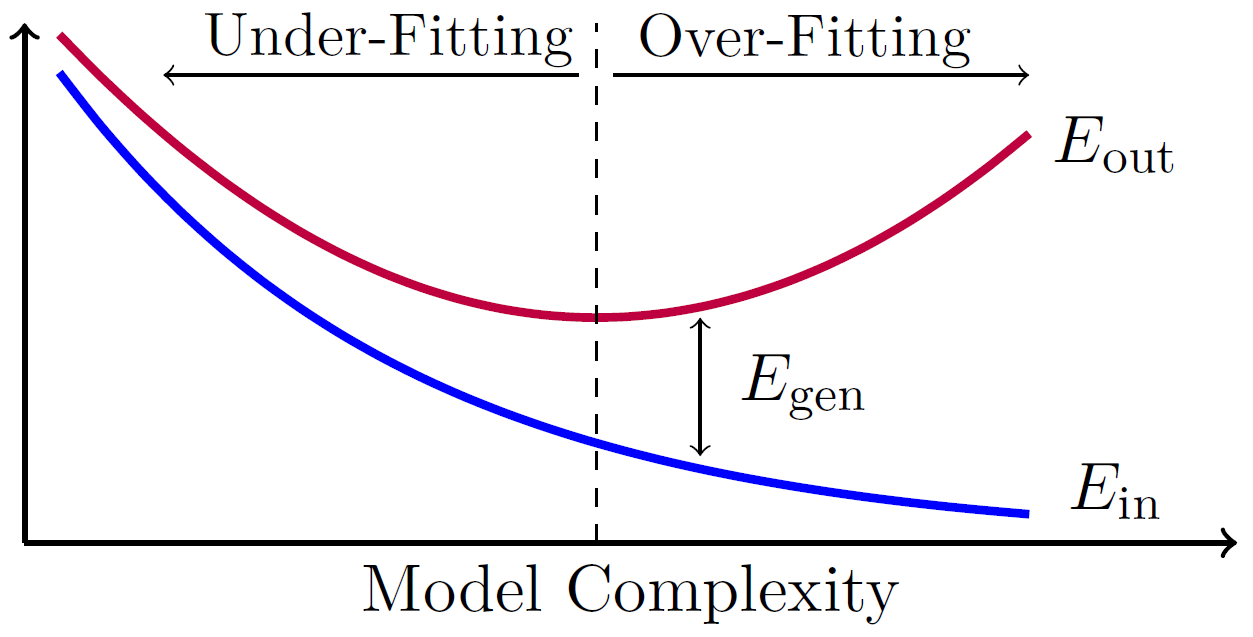
\includegraphics[width=0.6\textwidth]{images/overfitting.png}
	\caption{Overfitting and Underfitting}
	\label{fig:mesh1}
\end{figure}

\textbf{Regularization}: It refers to techniques that reduce over-fitting when learning with complex models.
\begin{equation}
	\mathcal{L}_{Reg} (\theta) = \mathcal{L} + \Omega(\theta)
\end{equation}

Popular regularziation methods can be listed as:
\begin{itemize}
	\item \textbf{Early Stop}
	\item \textbf{Dropout}
	\item \textbf{L1 Regularizer}: $\Omega(\theta) := \lambda_{Reg} | \theta | _2$
	\item \textbf{L2 Regularizer}: $\Omega(\theta) := \lambda_{Reg} || \theta || _2^2$
\end{itemize}

\section{Loss Functions}

\begin{itemize}
	\item \textbf{Mean Square Error}:
	\begin{equation}
		\hat{\theta} = \argmin_{\theta} ( Y - X \theta )^2
	\end{equation}
	\item \textbf{Cross Entropy}: Minimize Cross Entropy = Maximize Likelihood
	\begin{align}
		CE(\tilde{p}; p) &= - \sum_{y \in Y} \tilde{p} (y) \log p(y) \\
		&= - \mathbbm{1}_{y_i = 1} \log p_{Y|X} (1 | x_i) - \mathbbm{1}_{y_i = 0} \log p_{Y|X} (0 | x_i)
	\end{align}
	\item \textbf{Focal Loss function}
	\item \textbf{IoU Loss function}
	\item \textbf{Dice Loss function}
\end{itemize}

\section{Optimization Methods}

\section{Metrics}

\bibliographystyle{acm}
\bibliography{bibliography}
\end{document}